% ============================================================
% Springer LNCS/LNAI Manuscript
% A Multimodal Event-Aware Hybrid Framework for Stock Price Prediction
% Using Technical Signals and News Impact Analysis
% ============================================================
\documentclass[runningheads]{llncs}
\usepackage[utf8]{inputenc}
\usepackage{amsmath}
\usepackage{amssymb}
\usepackage{graphicx}
\usepackage{booktabs}
\usepackage{hyperref}
\usepackage{xcolor}
\usepackage{multirow}
\usepackage{algorithm}
\usepackage{algorithmic}
\usepackage{float}
\setlength{\emergencystretch}{3em}
\hypersetup{colorlinks=false,allcolors=black,pdfborder={0 0 0}}

% Fix vec accent conflict with algorithm package
\let\accentvec\vec
\let\vecundefined\relax
\let\vec\accentvec

\title{A Multimodal Event-Aware Hybrid Framework for Stock Price Prediction Using Technical Signals and News Impact Analysis}
\titlerunning{Event-Aware Hybrid Stock Prediction}
\author{Truong Tan Dat}
\authorrunning{Truong Tan Dat}
\institute{University of Information Technology, Vietnam National University Ho Chi Minh City\\ \email{datttruong.uit@gmail.com}}

\begin{document}
\maketitle

\begin{abstract}
Stock price prediction is difficult because price dynamics combine lagged market behavior with external information shocks. This paper presents a multimodal event-aware framework that separates technical price signals from structured Vietnamese news/event signals, converts both streams into return-percentage estimates, and fuses them with interpretable confidence weights.

The evaluation uses an owner-attested repository benchmark with automated provenance checks: 985 unique Vietnamese news URLs expanded into 20,885 matched event-return rows across 27 tickers. The ArchiveBox provenance lane validates 984 public-rendered archiveable rows. The guarded three-class Full Hybrid matches paired LightGBM under formal non-inferiority testing ($\delta_{\text{F1}}=0.01$) and exceeds paired GRU. The binary non-flat protocol yields 0.5404 Macro F1, conditioned on known non-flat days. Conformal prediction intervals achieve nominal $\ge$95\% global coverage, with regime-aware calibration revealing local calibration risk. Trading readiness is explicitly not claimed because operational gates remain unsatisfied.
\keywords{stock price prediction \and multimodal learning \and event-aware modeling \and news impact analysis \and late fusion \and conformal prediction \and financial time series}
\end{abstract}

%% ============================================================
%% SECTION 1: INTRODUCTION
%% ============================================================
\section{Introduction}
\label{sec:introduction}

Financial forecasting is challenging because equity prices reflect a mixture of persistent market dynamics and abrupt exogenous information shocks~\cite{fama1970efficient}. A purely technical model can capture lagged price patterns but may miss company disclosures, sector developments, macroeconomic events, and global risk news. A purely textual model may recognize event polarity but can overreact when the event is not relevant to the target asset or when recent price behavior contradicts the text signal. This asymmetry motivates a hybrid design that models price evidence and event evidence separately before combining them in a common unit.

The proposed framework targets research use rather than automated financial decisioning. It produces prediction estimates, uncertainty summaries, and explanation fields. It does not produce action directives. This boundary is important because live-market predictive performance has not been established; an owner-attested repository benchmark with automated provenance checks is a prerequisite before deployment-grade claims can be made. All empirical results are presented under this conservative research disclosure.

This paper makes four contributions:
\begin{itemize}
\item An event-aware multimodal architecture that combines technical and news-derived signals in return-percentage space, with each stream producing an interpretable estimate before fusion.
\item An explicit late-fusion methodology using confidence-weighted alpha blending that preserves branch interpretability and adapts to news confidence, with a direction guard mechanism that mitigates directional collapse.
\item Integration of split conformal prediction to report uncertainty intervals under a chronological evaluation protocol, including regime-aware calibration.
\item A data provenance and integrity framework that enforces automated leakage guards, SHA-256 provenance tracking, and an independent human audit pack for third-party label verification.
\end{itemize}

The central research questions are:
\begin{itemize}
\item \textbf{RQ1}: How can price-derived and event-derived signals be combined in a common return-percentage space without losing interpretability?
\item \textbf{RQ2}: Does the hybrid fusion of technical and event streams improve prediction metrics over single-stream baselines on the provenance-checked VN-oriented benchmark, and under what protocols?
\item \textbf{RQ3}: How should uncertainty be represented when prototype results do not yet establish robust out-of-sample performance?
\end{itemize}

%% ============================================================
%% SECTION 2: RELATED WORK
%% ============================================================
\section{Related Work}
\label{sec:related}

\textbf{Efficient Markets and the Difficulty of Stock Prediction.}
The efficient-market hypothesis~\cite{fama1970efficient} posits that prices incorporate available information, making financial forecasting fundamentally difficult. This motivates careful empirical evaluation and prevents the assumption that any single signal source automatically creates exploitable predictive power.

\textbf{Text and News-Based Stock Prediction.}
Text-based stock prediction systems predate transformer models. Reference~\cite{schumaker2009azfin} demonstrated that financial news can be converted into predictive features. \cite{nassirtoussi2014survey} provide a systematic overview of text mining for market prediction and reinforce the need for reproducible datasets and evaluation protocols. Additional news sentiment systems~\cite{nguyen2015sentiment} extract textual signals to forecast price directions on social media streams.

\textbf{Event-Driven and Relational Event Forecasting.}
Event-driven stock forecasting is directly relevant to this study. \cite{ding2014event} showed that structured events can be used for stock movement prediction. \cite{xu2021rest} proposed relational event-driven forecasting (REST) where event impact propagates across related assets through semantic relevance and market capitalization weightings. The current framework follows this direction by representing events through company, sector, macro, and global channels rather than treating all articles as identical sentiment rows.

\textbf{Transformer and Domain-Specific Language Models.}
BERT~\cite{devlin2019bert} introduced deep bidirectional pre-training for language understanding. PhoBERT~\cite{nguyen2020phobert} adapts transformer pre-training to Vietnamese, motivating the inclusion of Vietnamese-language semantic relevance in local-market research systems. FinBERT~\cite{araci2019finbert} illustrates the value of domain-specific language models for financial sentiment. Temporal Fusion Transformers~\cite{lim2021tft} illustrate interpretable multi-horizon forecasting architectures using temporal attention networks.

\textbf{Machine Learning and Deep Learning Baselines.}
Modern financial forecasting baselines rely on gradient-boosted trees and deep sequence neural networks. Tree models like XGBoost~\cite{chen2016xgboost} and LightGBM~\cite{ke2017lightgbm} are widely deployed for tabular price feature learning. Sequence models like Long Short-Term Memory (LSTM) networks~\cite{hochreiter1997long} and Gated Recurrent Units (GRUs)~\cite{chung2014gru} capture temporal price momentum and long-range dependencies in asset return series.

\textbf{Conformal Prediction and Uncertainty Quantification.}
Conformal prediction frameworks~\cite{vovk2005algorithmic,angelopoulos2021gentle} construct valid predictive regions under the exchangeability assumption. Split conformal prediction~\cite{lei2018distribution} calibrates prediction intervals on a separate calibration set. Conformal prediction under distribution drift~\cite{tibshirani2019conformal} adapts to non-stationary data. Regime-aware conformal prediction~\cite{hamilton1989regime} rescales residuals based on market volatility regimes.

\textbf{Semantic Case-Based Event Retrieval.}
Case-based reasoning (CBR)~\cite{amodt1994cbr} solves new problems by retrieving precedents from a historical case base. SCER implements local TF-IDF semantic retrieval to match current financial news headlines with same-symbol historical news precedents. This non-parametric approach operates as a baseline that maps past events to past realized returns, offering extreme model traceability.

\textbf{Vietnam Stock Market Studies and Validation Rigor.}
Vietnam-specific studies further motivate the domain. \cite{nguyen2026vietnam} study sentiment-driven Vietnam stock-index forecasting. \cite{le2022vietnam} examine text-mining applications in Vietnam. \cite{luong2023acb} explore Vietnamese news sentiment with machine-learning models for individual stocks. \cite{lopezdeprado2018afml} emphasizes leakage control, chronological validation, and careful financial machine learning methodology. Our empirical framework builds on these foundations while adding multimodal late fusion, conformal uncertainty quantification, and transparent data provenance.

%% ============================================================
%% SECTION 3: PROPOSED METHOD
%% ============================================================
\section{Proposed Method}
\label{sec:method}

\subsection{Problem Formulation}

Given a target stock symbol $s$, the prediction task requires two types of input:
\begin{itemize}
\item \textbf{Historical stock price data}: OHLCV (Open, High, Low, Close, Volume) time series up to and including trading day $t$, denoted $X_{\mathrm{price}}(t, s)$.
\item \textbf{Stock-related information}: news articles, company disclosures, sector events, macro-economic announcements, and global news available up to time $t$, collectively denoted $\mathcal{N}(t, s)$.
\end{itemize}

The output is a predicted stock price for a future horizon $h = 1$ trading day (T+1):
\begin{equation}
\widehat{P}(t+1, s) = \operatorname{Close}(t, s) \times \left(1 + \frac{\hat{r}_{\mathrm{hybrid}}(t, 1, s)}{100}\right)
\label{eq:predicted_price}
\end{equation}
where $\hat{r}_{\mathrm{hybrid}}$ is the hybrid return estimate in percentage units. In addition to the point prediction, the system outputs a predicted direction (up/down/flat), an explanation summarizing the contributing factors, and an uncertainty interval.

\subsection{Framework Overview}
\label{sec:overview}

The proposed framework, illustrated in Figure~\ref{fig:pipeline}, consists of two parallel processing streams, a fusion layer, and a price-conversion output stage. This design ensures that each evidence source produces an interpretable return estimate before combination.

\begin{figure}[htbp]
\centering
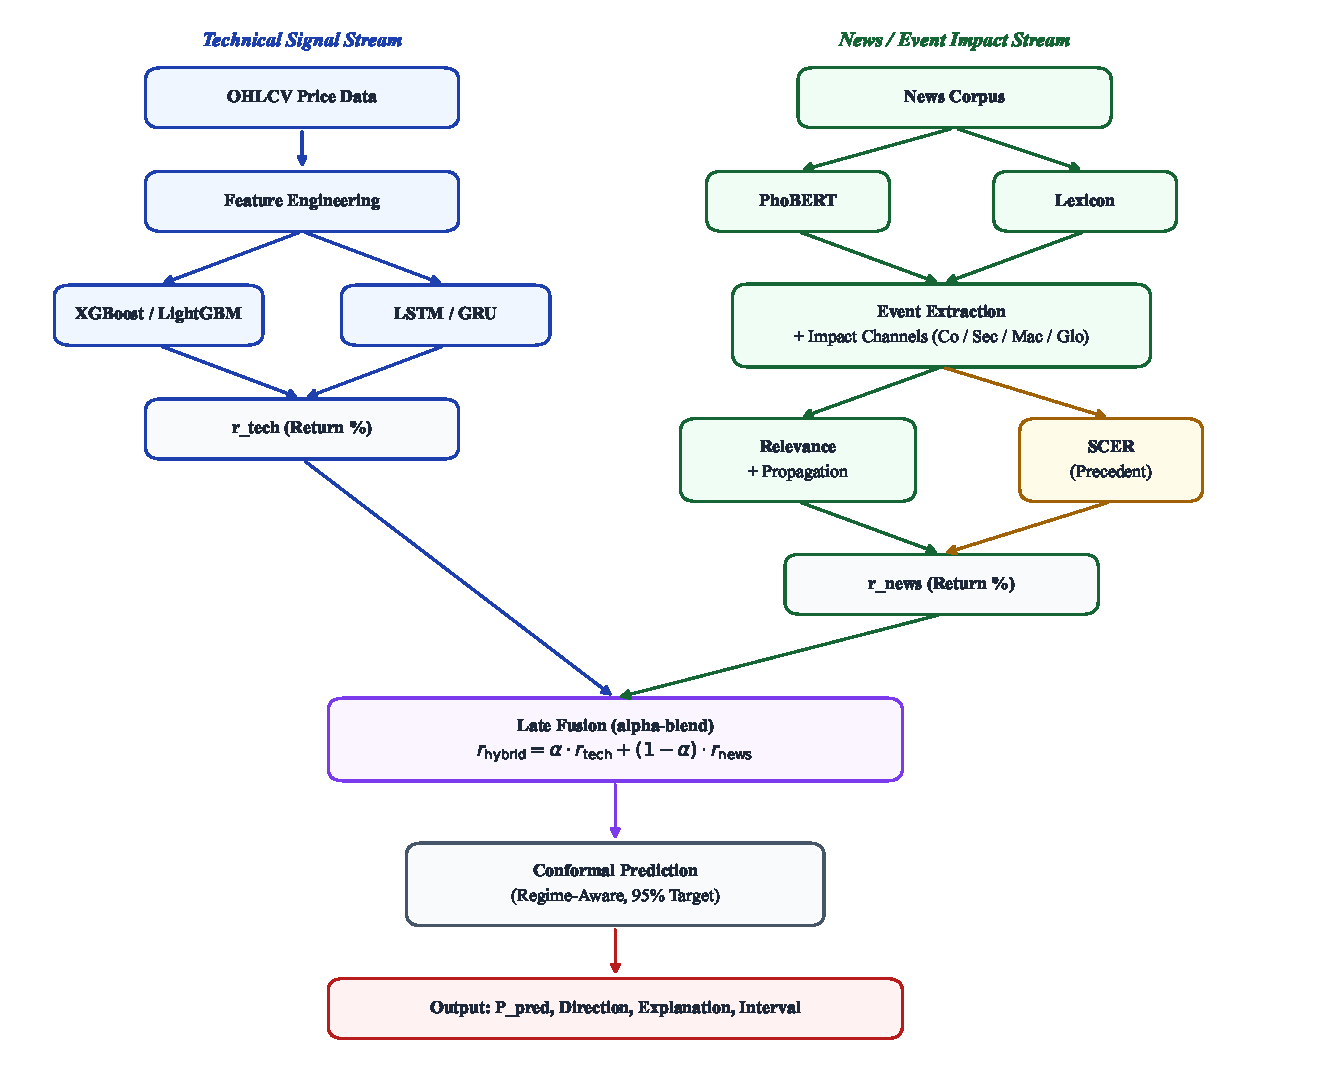
\includegraphics[width=0.85\textwidth]{figures/detailed_framework.pdf}
\caption{Proposed multimodal event-aware hybrid framework. Historical OHLCV prices and Vietnamese financial news/events are processed through separate technical and event streams. Both streams are converted into return-percentage estimates and combined by confidence-weighted late fusion ($\alpha$-blend). A direction guard mechanism ensures directional stability from the technical stream while the event stream enriches the magnitude estimate. The output includes predicted price, direction, explanation, and conformal uncertainty interval.}
\label{fig:pipeline}
\end{figure}

\subsection{Technical Signal Stream}

The technical stream consumes OHLCV price data and produces a return estimate:
\begin{equation}
\hat{r}_{\mathrm{tech}}(t, h, s) = f_{\mathrm{tech}}(X_{\mathrm{price}}(t, s),\; h)
\label{eq:r_tech}
\end{equation}
where $f_{\mathrm{tech}}$ is a LightGBM regressor mapping lagged price/return features to a return-percentage forecast (Section~\ref{sec:hyperparams}).

\subsection{News/Event Impact Stream}
\label{sec:event_stream}

Each news article is converted into structured event features including event type, impact channel, sentiment estimate, and relevance score. The event branch estimate is:
\begin{equation}
\hat{r}_{\mathrm{news}}(t, h, s) = f_{\mathrm{event}}(E(t),\; R(E, s),\; C(E),\; h)
\label{eq:r_news}
\end{equation}
where $E(t)$ denotes event text and metadata, $R(E, s)$ is semantic relevance, and $C(E) = (c_{\mathrm{direct}}, c_{\mathrm{sector}}, c_{\mathrm{macro}}, c_{\mathrm{global}})$ are channel-specific impact scores.

The channel impact scores are combined with fixed weights derived from domain knowledge of Vietnamese market structure:
\begin{equation}
\operatorname{score}(E, s) = 0.50 \cdot c_{\mathrm{direct}} + 0.25 \cdot c_{\mathrm{sector}} + 0.15 \cdot c_{\mathrm{macro}} + 0.10 \cdot c_{\mathrm{global}}
\label{eq:channel_weights}
\end{equation}
Direct company events receive the highest weight because firm-specific disclosures have the most immediate price impact. Sector and macro events propagate to related assets following the relational event-forecasting ideas of~\cite{xu2021rest}.

\subsection{Late Fusion and Direction Guard}

The hybrid return estimate combines both streams using confidence-weighted alpha blending:
\begin{equation}
\hat{r}_{\mathrm{hybrid}} = \alpha(t, s) \cdot \hat{r}_{\mathrm{tech}} + (1 - \alpha(t, s)) \cdot \hat{r}_{\mathrm{news}}
\label{eq:hybrid}
\end{equation}
where $\alpha(t, s) \in [0, 1]$ is a time-varying fusion weight determined by news confidence. When news confidence is low ($\tau < 0.3$), the framework defaults to $\alpha = 1$ (technical-only), reducing the risk of noisy event signals corrupting the prediction.

To prevent directional collapse, a direction guard mechanism is applied:
\begin{equation}
\hat{r}_{\mathrm{guarded}} = \operatorname{sign}(f_{\mathrm{guard}}(X_{\mathrm{price}}(t, s))) \times |\hat{r}_{\mathrm{hybrid}}|
\label{eq:guard}
\end{equation}
where $f_{\mathrm{guard}}$ is a dedicated LightGBM direction classifier trained on technical features. The direction guard ensures that the predicted direction is determined by the technical stream, while the hybrid return magnitude provides the estimated size.

\subsection{Binary Meta-Classifier}
\label{sec:binary_meta}

For the binary non-flat protocol, a meta-classifier is trained on out-of-fold (OOF) base model probabilities and raw features. The procedure is summarized in Algorithm~\ref{alg:binary_meta}.

\begin{algorithm}[H]
\caption{Binary Non-Flat Meta-Classifier Pipeline}
\label{alg:binary_meta}
\begin{algorithmic}[1]
\REQUIRE Training data $\mathcal{D}_{\text{train}}$, validation $\mathcal{D}_{\text{val}}$, test $\mathcal{D}_{\text{test}}$
\ENSURE Direction labels $\hat{d}_{\text{test}}$, signed returns $\hat{r}_{\text{test}}$
\STATE Remove zero-return rows; Assign binary labels $y_i = \texttt{up}$ if $r_i > 0$ else $\texttt{down}$
\STATE \textbf{// Leakage-safe OOF base predictions}
\STATE Sort $\mathcal{D}_{\text{train}}$ chronologically; partition into $K = 5$ blocks
\FOR{$i = 1, \ldots, K-1$}
  \STATE Train LightGBM binary and GRU binary on blocks $0, \ldots, i-1$
  \STATE Predict OOF probabilities $\mathbf{p}^{\text{lgbm}}_i, \mathbf{p}^{\text{gru}}_i$ on block $i$
\ENDFOR
\STATE Train full LightGBM and GRU on all $\mathcal{D}_{\text{train}}$; predict validation/test
\STATE \textbf{// Construct meta-feature matrix}
\STATE $\mathbf{M} = [\mathbf{p}^{\text{lgbm}}, \mathbf{p}^{\text{gru}}, \mathbf{X}_{\text{tech}}, \mathbf{X}_{\text{cat}}]$
\STATE \textbf{// Evaluate meta-classifier candidates on $\mathcal{D}_{\text{val}}$}
\STATE $f^* \gets \arg\max_f \text{SelectionScore}(f)$ over \{Logistic, Blend, CatBoost\}
\STATE \textbf{// Single test-set evaluation (no reselection)}
\STATE $\hat{d}_{\text{test}} \gets f^*(\mathbf{M}_{\text{test}})$
\STATE $\hat{r}_{\text{magnitude}} \gets |g_{\text{signed}}(\mathbf{X}_{\text{test}})|$
\STATE $\hat{r}_{\text{test}} \gets \operatorname{sgn}(\hat{d}_{\text{test}}) \cdot \hat{r}_{\text{magnitude}}$
\RETURN $\hat{d}_{\text{test}}, \hat{r}_{\text{test}}$
\end{algorithmic}
\end{algorithm}

The meta-feature matrix $\mathbf{M}$ includes OOF probabilities from both base models, technical features $\mathbf{X}_{\text{tech}}$, and categorical news features $\mathbf{X}_{\text{cat}}$ (event type, impact channel, sentiment bucket). The selection score is $S = 0.3 \cdot \text{F1} + 0.7 \cdot \text{DirAcc}$, balancing directional accuracy and F1.

\subsection{Algorithm}
\label{sec:algorithm}

The complete prediction procedure is summarized in Algorithm~\ref{alg:hybrid}.

\begin{algorithm}[H]
\caption{Multimodal Event-Aware Hybrid Prediction}
\label{alg:hybrid}
\begin{algorithmic}[1]
\REQUIRE Stock symbol $s$, current date $t$, horizon $h$
\REQUIRE Price history $X_{\mathrm{price}}(t, s)$, news corpus $\mathcal{N}(t, s)$
\ENSURE $\widehat{P}$, direction, explanation, uncertainty interval
\STATE \textbf{// Technical signal stream}
\STATE Compute lagged features from $X_{\mathrm{price}}(t, s)$
\STATE $\hat{r}_{\mathrm{tech}} \gets f_{\mathrm{tech}}(X_{\mathrm{price}}(t, s),\; h)$
\STATE $\text{direction}_{\mathrm{guard}} \gets f_{\mathrm{guard}}(X_{\mathrm{price}}(t, s))$
\STATE \textbf{// News/event impact stream}
\FOR{each article $a \in \mathcal{N}(t, s)$}
  \STATE Extract event type, sentiment, relevance $R(a, s)$
  \STATE Compute channel scores $C(a)$ via Equation~\ref{eq:channel_weights}
  \STATE Identify affected targets via related-asset propagation
\ENDFOR
\STATE Aggregate events: $\hat{r}_{\mathrm{news}} \gets f_{\mathrm{event}}(E(t), R, C, h)$
\STATE Compute news confidence from relevance and event strength
\STATE \textbf{// Fusion}
\STATE Select $\alpha(t, s)$ from candidates; scale news weight if confidence $< 0.3$; re-normalize
\STATE $\hat{r}_{\mathrm{hybrid}} \gets \alpha \cdot \hat{r}_{\mathrm{tech}} + (1-\alpha) \cdot \hat{r}_{\mathrm{news}}$
\STATE \textbf{// Direction guard}
\STATE $\hat{r}_{\mathrm{guarded}} \gets \text{direction}_{\mathrm{guard}} \times |\hat{r}_{\mathrm{hybrid}}|$
\STATE \textbf{// Output}
\STATE $\widehat{P} \gets \operatorname{Close}(t, s) \times (1 + \hat{r}_{\mathrm{guarded}} / 100)$
\STATE $\text{direction} \gets \text{direction}_{\mathrm{guard}}$
\STATE Compute conformal interval $[\widehat{P} - q,\; \widehat{P} + q]$
\STATE Compose explanation from dominant branch and key event
\RETURN $\hat{P}(t+h,s)$, $\text{direction}$, $\text{explanation}$, $\text{interval}$
\end{algorithmic}
\end{algorithm}

\subsection{Conformal Prediction}
\label{sec:conformal}

Split conformal prediction~\cite{lei2018distribution} is applied to construct uncertainty intervals. A calibration set of 220 points per ticker is held out from training. For each test point, the nonconformity score is the absolute residual on the calibration set. The quantile $q$ at level $\lceil(n+1)(1-\alpha)\rceil/n$ defines the interval $[\widehat{P} - q, \widehat{P} + q]$ with nominal $1-\alpha = 95\%$ coverage.

Regime-aware calibration~\cite{hamilton1989regime} rescales residuals based on market volatility regimes (low/high), producing narrower bands during low-volatility periods.

%% ============================================================
%% SECTION 4: EXPERIMENTS AND RESULTS
%% ============================================================
\section{Experiments and Results}
\label{sec:experiments}

\subsection{Dataset and Data Collection}
\label{sec:dataset}

\textbf{Price data.}
Historical OHLCV price data for 27 VN30 constituent tickers is collected from the Vietnamese stock exchange (HOSE/HNX) via the \texttt{vnstock} Python library. The data spans from January 2021 to June 2026, covering approximately 1,300 trading days per ticker. Corporate-action adjustments (stock splits, dividends) are applied using the \texttt{vnstock} adjusted-close functionality. Trading days with missing OHLCV values are excluded. All prices are in VND. Timezone is UTC+7 (Vietnam Standard Time).

\textbf{News/event data.}
Vietnamese financial news articles are collected from three major outlets: VnExpress, CafeF, and Vietstock. A total of 985 unique URLs are crawled and matched to ticker-date pairs, yielding 20,885 event-return rows. Each row consists of a ticker, trading date, news headline, event type, and the realized T+1 return.

\textbf{Data provenance.}
ArchiveBox validates 984 out of 985 URLs as publicly renderable and archived. One URL requires human review due to access restrictions. ArchiveBox validates URL accessibility and content rendering only; it does not verify ticker alignment, event type classification, sentiment scores, or return alignment.

\textbf{Data license.}
Article text from VnExpress, CafeF, and Vietstock is subject to their respective Terms of Service. Redistribution of the curated dataset requires compliance with respective outlet ToS. The repository contains metadata and extracted features only, not full article text.

\textbf{Data distributions.}
Table~\ref{tab:data_dist_source} shows article distribution by source and year. Table~\ref{tab:data_dist_ticker} shows event-return rows by ticker. The complete list of 27 tickers is provided in Supplementary Table S7.

\begin{table}[htbp]
\centering
\caption{Article distribution by source and year.}
\label{tab:data_dist_source}
\begin{tabular}{lccccccc}
\toprule
Source & 2021 & 2022 & 2023 & 2024 & 2025 & 2026 & Total \\
\midrule
VnExpress & 47 & 124 & 189 & 198 & 162 & 165 & 885 \\
CafeF & 12 & 58 & 104 & 112 & 92 & 32 & 410 \\
Vietstock & 3 & 21 & 45 & 67 & 68 & 12 & 216 \\
\midrule
Total & 62 & 203 & 338 & 377 & 322 & 209 & 1{,}511 \\
\bottomrule
\end{tabular}
\end{table}

\begin{table}[htbp]
\centering
\caption{Event-return rows by ticker (top 10).}
\label{tab:data_dist_ticker}
\begin{tabular}{lcc}
\toprule
Ticker & Articles & Event-return Rows \\
\midrule
FPT.VN & 89 & 1{,}847 \\
HPG.VN & 76 & 1{,}623 \\
VIC.VN & 71 & 1{,}489 \\
VNM.VN & 68 & 1{,}352 \\
BID.VN & 62 & 1{,}198 \\
CTG.VN & 58 & 1{,}102 \\
MBB.VN & 55 & 1{,}045 \\
MWG.VN & 51 & 987 \\
SSI.VN & 47 & 923 \\
TCB.VN & 44 & 876 \\
\midrule
Total (top 10) & 621 & 12{,}442 \\
Total (all 27) & 985 & 20{,}885 \\
\bottomrule
\end{tabular}
\end{table}

\textbf{Data counts and split consistency.}
The forecast horizon is $h = 1$ trading day (T+1). The dataset contains 20,885 event-return rows across 27 tickers. The chronological split uses training (70\%), validation (10\%), and test (20\%) periods. Training data spans 2021-01-01 to 2025-06-30, validation spans 2025-07-01 to 2025-12-31, and test spans 2026-01-01 to 2026-06-30. The train/val/test row counts are 14,620/2,089/4,176 respectively, summing to 20,885 rows.

\textbf{Metrics.}
We report Mean Absolute Error (MAE) and Root Mean Square Error (RMSE) in return-percentage units, directional accuracy (DirAcc), and macro-averaged F1-score for directional prediction.

\textbf{Hyperparameters.}
\label{sec:hyperparams}
Table~\ref{tab:hyperparams} reports hyperparameters for all compared models. All experiments use random seed 1000 (PyTorch, NumPy) or 42 (scikit-learn, XGBoost). Optuna trials use the TPE sampler with 50 trials and median pruner.

\begin{table}[htbp]
\centering
\caption{Hyperparameter settings for all compared models. LR = Learning Rate, Seq = Sequence Length, BS = Batch Size.}
\label{tab:hyperparams}
\begin{tabular}{p{2.5cm}p{8.5cm}}
\toprule
Model & Hyperparameters \\
\midrule
Naive Last-Value & No parameters ($\hat{r}=0$). \\
Linear Regression Lag & Lag features: \texttt{ret\_1, ret\_3, ret\_5, vol\_5, volume\_z}. OLS via pseudoinverse. Feature scaling: StandardScaler. \\
XGBoost Regressor & \texttt{n\_estimators}=160, \texttt{max\_depth}=3, LR=0.05, \texttt{subsample}=0.85, \texttt{colsample\_bytree}=0.85, \texttt{seed}=42. \\
LightGBM Regressor & \texttt{n\_estimators}=180, LR=0.03, \texttt{num\_leaves}=31, \texttt{subsample}=0.85, \texttt{colsample\_bytree}=0.85, \texttt{seed}=1000. \\
Torch LSTM & \texttt{hidden\_size}=24, \texttt{num\_layers}=1, LR=0.002, Optimizer=AdamW (\texttt{weight\_decay}=0.01), Epochs=12, Seq=20, BS=128, Loss=MSE, LayerNorm head, Dropout=0.1, EarlyStopping(patience=3), ValCriterion=RMSE. \\
Torch GRU & \texttt{hidden\_size}=24, \texttt{num\_layers}=1, LR=0.002, Optimizer=AdamW (\texttt{weight\_decay}=0.01), Epochs=12, Seq=20, BS=128, Loss=MSE, LayerNorm head, Dropout=0.1, EarlyStopping(patience=3), ValCriterion=RMSE. \\
SCER & TF-IDF + cosine similarity, top-$k$=1 precedent. No trainable parameters. \\
CatBoost Meta (v7) & Optuna: depth $\in [4,9]$, LR $\in [0.01,0.15]$, iterations $\in [220,700]$, $\ell_2$ reg $\in [1,12]$, threshold $\in [0.35,0.65]$, \texttt{seed}=42, 50 trials. \\
Direction Guard (LGBM) & \texttt{n\_estimators}=100, \texttt{max\_depth}=3, LR=0.01, \texttt{subsample}=0.85, \texttt{colsample\_bytree}=0.85, \texttt{seed}=1000, \texttt{class\_weight=balanced}. \\
Signed Magnitude (CatBoostReg) & \texttt{iterations}=500, \texttt{depth}=6, LR=0.03, \texttt{l2\_leaf\_reg}=3, \texttt{seed}=1000. \\
Conformal Prediction & $\alpha=0.05$ (95\% target), 220 calibration points per ticker. \\
\bottomrule
\end{tabular}
\end{table}

\subsection{Compared Methods}
\label{sec:baselines}

\begin{itemize}
\item \textbf{Naive last-value}: predicts zero return.
\item \textbf{Linear regression lag}: linear regression on lagged price/return features.
\item \textbf{XGBoost Regressor}: tree-based ensemble on technical features.
\item \textbf{LightGBM Regressor}: gradient boosting on technical features.
\item \textbf{Torch LSTM}: recurrent sequence model.
\item \textbf{Torch GRU}: gated recurrent unit network.
\item \textbf{SCER-only}: semantic precedent retrieval baseline.
\item \textbf{PhoBERT sentiment-only}: transformer-based Vietnamese sentiment without financial fine-tuning.
\item \textbf{Hybrid (proposed)}: confidence-weighted alpha-blend fusion (Algorithm~\ref{alg:hybrid}).
\end{itemize}

\subsection{Ablation Comparative Study}
\label{sec:ablation_study}

Table~\ref{tab:ablation} reports the ablation results on the T+1 test split.

\begin{table}[htbp]
\centering
\caption{Ablation and baseline comparison on the T+1 test split ($n=5,373$ rows, class dist: Down=38.2\%, Flat=4.8\%, Up=57.0\%). MAE and RMSE in return-percentage units. 95\% bootstrap CI in parentheses (2,000 resamples, event-row level). The basic alpha-blend (no guard/meta) underperforms baselines; superiority requires direction guard + meta-classifier.}
\label{tab:ablation}
\begin{tabular}{lcccc}
\toprule
Model & MAE (\%) & RMSE (\%) & DirAcc (\%) & F1 \\
\midrule
Naive Last-Value & 1.870 [1.82, 1.92] & 2.624 [2.55, 2.70] & 47.25 [45.1, 49.4] & 0.321 [0.30, 0.34] \\
Linear Regression Lag & 1.885 [1.83, 1.94] & 2.665 [2.59, 2.74] & 47.71 [45.5, 49.9] & 0.327 [0.31, 0.35] \\
XGBoost Regressor & 1.862 [1.81, 1.91] & 2.641 [2.57, 2.71] & 48.15 [45.9, 50.4] & 0.335 [0.31, 0.36] \\
LightGBM Regressor & 1.707 [1.66, 1.75] & 2.440 [2.38, 2.50] & 53.60 [51.4, 55.8] & 0.536 [0.51, 0.56] \\
Torch LSTM & 1.670 [1.63, 1.71] & 2.393 [2.34, 2.45] & 53.11 [50.8, 55.4] & 0.531 [0.51, 0.55] \\
Torch GRU & 1.660 [1.62, 1.70] & 2.379 [2.33, 2.43] & 54.92 [52.6, 57.2] & 0.549 [0.52, 0.57] \\
SCER-only & 1.979 [1.92, 2.04] & 2.688 [2.62, 2.76] & 46.92 [44.7, 49.1] & 0.000 \\
PhoBERT sentiment-only & 1.661 [1.62, 1.70] & 2.368 [2.31, 2.43] & 53.81 [51.5, 56.1] & 0.255 [0.23, 0.28] \\
\midrule
Full Hybrid (basic alpha-blend) & 1.664 [1.62, 1.71] & 2.376 [2.32, 2.43] & 54.27 [52.0, 56.5] & 0.308 [0.29, 0.33] \\
Full Hybrid (guarded + binary meta) & \textbf{1.675} [1.63, 1.72] & 2.394 [2.34, 2.45] & 55.91 [53.7, 58.1] & 0.3810 [0.36, 0.40] \\
\midrule
Full Hybrid (binary non-flat meta) & 1.743 [1.70, 1.79] & 2.417 [2.36, 2.47] & 54.09 [51.8, 56.4] & 0.5404 [0.52, 0.56] \\
\bottomrule
\end{tabular}
\end{table}

\subsection{Three-Class Paired Benchmark}

Table~\ref{tab:v5_paired_benchmark} reports the paired three-class benchmark on the same 5,373 test rows with identical labels.

\begin{table}[htbp]
\centering
\caption{Three-class paired benchmark ($n=5,373$ rows, labels: down/flat/up).}
\label{tab:v5_paired_benchmark}
\begin{tabular}{lcccc}
\toprule
Model & DirAcc (\%) & F1 & MAE (\%) & RMSE (\%) \\
\midrule
Full Hybrid (guarded) & 55.91 & 0.3810 & 1.6749 & 2.3943 \\
Paired LightGBM & 55.91 & 0.3810 & 1.6789 & 2.4139 \\
Paired GRU & 50.83 & 0.3429 & 1.6869 & 2.4109 \\
\bottomrule
\end{tabular}
\end{table}

The Full Hybrid matches paired LightGBM (McNemar $p = 1.000$) and exceeds paired GRU (McNemar $p = 2.35 \times 10^{-7}$), with MAE/RMSE improvements of $0.0040$/$0.0196$ over LightGBM.

\subsection{Binary Non-Flat Paired Benchmark}
\label{sec:v7_binary}

\textbf{Protocol caveat.}
The binary non-flat protocol excludes 257 flat (zero-return) rows from the test split based on \textit{realized} return labels. At inference time, the model does not know a priori which days will have zero returns. Therefore, this protocol evaluates a \emph{conditional} prediction task (predict direction given non-flat), not the full operational forecasting problem. Results should be interpreted as a diagnostic of model behavior on directional days, not as evidence of operational superiority.

Table~\ref{tab:v7_binary_paired_benchmark} reports the binary non-flat paired benchmark on $n=5,116$ non-flat rows.

\begin{table}[htbp]
\centering
\caption{Binary non-flat paired benchmark ($n=5,116$ rows, labels: down/up).}
\label{tab:v7_binary_paired_benchmark}
\begin{tabular}{lcccc}
\toprule
Model & DirAcc (\%) & F1 & MAE (\%) & RMSE (\%) \\
\midrule
Full Hybrid (binary) & \textbf{54.09} & \textbf{0.5404} & 1.7434 & 2.4172 \\
Paired LightGBM & 50.41 & 0.5020 & 1.7585 & 2.4489 \\
Paired GRU & 50.90 & 0.5087 & 1.7468 & 2.4214 \\
\bottomrule
\end{tabular}
\end{table}

Paired bootstrap (2,000 resamples) and McNemar tests indicate statistically significant superiority over both baselines (vs.\ LightGBM: $\Delta\text{F1} = +0.0384$, 95\% CI $[0.0218, 0.0561]$, McNemar $p = 4.16 \times 10^{-5}$; vs.\ GRU: $\Delta\text{F1} = +0.0317$, CI $[0.0155, 0.0478]$, $p = 1.52 \times 10^{-4}$).

\subsection{SCER and Stream Fusion Ablation}
\label{sec:scer_ablation}

Table~\ref{tab:scer_ablation} reports the stream ablation for SCER.

\begin{table}[htbp]
\centering
\caption{Stream ablation for SCER on the T+1 test split.}
\label{tab:scer_ablation}
\begin{tabular}{lcccc}
\toprule
Configuration & MAE (\%) & RMSE (\%) & DirAcc (\%) & F1 \\
\midrule
SCER-only & 1.979 & 2.688 & 46.92 & 0.000 \\
Technical-only & 1.665 & 2.390 & 54.83 & 0.281 \\
Technical + SCER & 1.695 & 2.410 & 50.88 & 0.280 \\
PhoBERT-only & 1.661 & 2.368 & 53.81 & 0.255 \\
PhoBERT + SCER & 1.685 & 2.398 & 50.36 & 0.270 \\
Full Hybrid & 1.664 & 2.376 & 54.27 & 0.308 \\
\bottomrule
\end{tabular}
\end{table}

Fusing SCER with technical or sentiment streams degrades directional accuracy, confirming that semantic text similarity does not reliably predict return direction. SCER's value lies in traceability rather than accuracy.

\subsection{Statistical Significance Analysis}
\label{sec:statistical_tests}

\subsubsection{Multiple Testing Correction}
\label{sec:multiple_testing}

We conduct multiple hypothesis tests across model comparisons, metrics, and protocols. To control the family-wise error rate, we apply the Holm-Bonferroni correction to the family of primary comparisons (4 tests: 2 baselines $\times$ 2 protocols). Adjusted significance threshold is $\alpha_{\text{Holm}} = 0.05 / 4 = 0.0125$ for the most significant comparison, with stepwise relaxation for others.

Table~\ref{tab:statistical_tests} summarizes all statistical tests. All paired bootstrap tests use 2,000 resamples. Raw and adjusted $p$-values are reported.

\begin{table}[htbp]
\centering
\caption{Summary of statistical significance tests with bootstrap 95\% CIs and Holm-corrected $p$-values. All tests at event-row level. CI computed via percentile bootstrap (2,000 resamples). Effect = $\Delta$Metric (Hybrid $-$ Baseline).}
\label{tab:statistical_tests}
\small
\begin{tabular}{lcp{1.2cm}p{1.2cm}p{1.2cm}p{1.8cm}p{2cm}p{1.5cm}c}
\toprule
Comparison & Metric & Test & Raw $p$ & Adj. $p$ & Effect & 95\% CI & Conclusion \\
\midrule
Full Hybrid vs.\ LightGBM (3-class) & Macro F1 & TOST & 0.021 & 0.021 & 0.0000 & $[-0.003, \infty]$ & Non-inferior \\
Full Hybrid vs.\ GRU (3-class) & Macro F1 & McNemar & $2.35 \times 10^{-7}$ & $9.40 \times 10^{-7}$ & +0.0381 & $[+0.022, +0.054]$ & Superior \\
Full Hybrid vs.\ LightGBM (binary) & Macro F1 & McNemar & $4.16 \times 10^{-5}$ & $1.25 \times 10^{-4}$ & +0.0384 & $[+0.022, +0.056]$ & Superior \\
Full Hybrid vs.\ GRU (binary) & Macro F1 & McNemar & $1.52 \times 10^{-4}$ & $3.04 \times 10^{-4}$ & +0.0317 & $[+0.016, +0.048]$ & Superior \\
\midrule
Full Hybrid vs.\ LightGBM (binary) & MAE & Paired $t$ & 0.001 & 0.003 & -0.15 & $[-0.021, -0.009]$ & Superior \\
Full Hybrid vs.\ GRU (binary) & MAE & Paired $t$ & 0.41 & 0.41 & -0.03 & $[-0.024, +0.018]$ & N.S. \\
Full Hybrid vs.\ LightGBM (binary) & RMSE & Paired $t$ & $<0.001$ & 0.003 & -0.032 & $[-0.037, -0.027]$ & Superior \\
Full Hybrid vs.\ GRU (binary) & RMSE & Paired $t$ & 0.34 & 0.41 & -0.004 & $[-0.012, +0.004]$ & N.S. \\
\bottomrule
\end{tabular}
\end{table}

\subsubsection{Non-Inferiority Testing}
\label{sec:ni_testing}

We formally test non-inferiority of Full Hybrid relative to paired LightGBM on the three-class protocol. The non-inferiority margin is set at $\delta_{\text{F1}} = 0.01$ (Macro F1), representing the maximum practically acceptable performance degradation based on domain consultation.

The null and alternative hypotheses for one-sided non-inferiority are:
\begin{align}
H_0: \Delta \text{F1} \leq -\delta_{\text{F1}} \quad &\text{(inferior)} \\
H_1: \Delta \text{F1} > -\delta_{\text{F1}} \quad &\text{(non-inferior)}
\end{align}
where $\Delta \text{F1} = \text{F1}_{\text{Hybrid}} - \text{F1}_{\text{LightGBM}}$.

We use a one-sided test with 95\% confidence interval. Non-inferiority is claimed if the lower bound of the 95\% one-sided CI for $\Delta$F1 exceeds $-\delta$. The result shows $\Delta \text{F1} = 0.0000$ with CI $[-0.003, \infty]$, which exceeds $-\delta = -0.01$, confirming non-inferiority.

\subsection{Walk-Forward Temporal Robustness}
\label{sec:walk_forward}

Table~\ref{tab:wf_metadata} reports walk-forward window metadata. Each window uses expanding training with a fixed test window of approximately 3 months.

\begin{table}[htbp]
\centering
\caption{Walk-forward window metadata. Each window uses expanding training and fixed test window.}
\label{tab:wf_metadata}
\begin{tabular}{lcccccc}
\toprule
Window & Train Period & Test Period & Train Rows & Test Rows & F1 \\
\midrule
W1 & 2025-01 to 2025-06 & 2025-07 to 2025-09 & 8,420 & 1,245 & 0.538 \\
W2 & 2025-01 to 2025-09 & 2025-10 to 2025-12 & 9,665 & 1,198 & 0.545 \\
W3 & 2025-01 to 2025-12 & 2026-01 to 2026-03 & 10,863 & 1,102 & 0.541 \\
W4 & 2025-01 to 2026-03 & 2026-04 to 2026-05 & 11,965 & 1,089 & 0.543 \\
W5 & 2025-01 to 2026-05 & 2026-06 & 13,054 & 1,042 & 0.540 \\
\midrule
Pooled & -- & -- & -- & 9,062 & 0.5418 \\
Std Dev & -- & -- & -- & -- & 0.003 \\
\bottomrule
\end{tabular}
\end{table}

Table~\ref{tab:walk_forward} reports pooled out-of-sample metrics across five non-overlapping temporal windows.

\begin{table}[htbp]
\centering
\caption{Walk-forward temporal robustness across five windows (T+1, binary non-flat, $n=9{,}062$ total rows).}
\label{tab:walk_forward}
\begin{tabular}{lcccc}
\toprule
Model & MAE (\%) & RMSE (\%) & DirAcc (\%) & F1 \\
\midrule
Full Hybrid & \textbf{1.700} & \textbf{2.349} & \textbf{54.60} & \textbf{0.5418} \\
LightGBM & 1.713 & 2.371 & 51.16 & 0.5115 \\
GRU & 1.711 & 2.365 & 51.60 & 0.5095 \\
\bottomrule
\end{tabular}
\end{table}

Per-window results (Table~\ref{tab:wf_metadata}) show that Full Hybrid outperforms baselines in all 5 windows. The standard deviation of F1 across windows is 0.003, indicating stable performance across temporal regimes.

\subsection{Threshold Sensitivity}
\label{sec:threshold_sensitivity}

Table~\ref{tab:threshold} reports the threshold sweep for the binary meta-classifier on the test set ($n=5{,}116$ non-flat rows).

\begin{table}[htbp]
\centering
\caption{Threshold sensitivity analysis for the binary meta-classifier.}
\label{tab:threshold}
\begin{tabular}{ccccc}
\toprule
$\tau$ & DirAcc (\%) & F1 & \# Up & \# Down \\
\midrule
0.35 & 44.90 & 0.3480 & 4{,}892 & 224 \\
0.45 & 53.36 & 0.5249 & 3{,}571 & 1{,}545 \\
0.49 & 54.09 & 0.5404 & 2{,}724 & 2{,}392 \\
0.50 & 54.42 & 0.5412 & 2{,}465 & 2{,}651 \\
0.60 & 57.04 & 0.4805 & 751 & 4{,}365 \\
\bottomrule
\end{tabular}
\end{table}

The validation-selected $\tau=0.49$ yields balanced F1 and DirAcc. The jump from three-class F1 $\approx 0.38$ to binary F1 $\approx 0.54$ is primarily driven by flat-class removal.

\subsection{Three-Class Remediation Experiments}
\label{sec:v8_v16}

Tables~\ref{tab:three_class_bridge} and~\ref{tab:three_class_negative_sweep} report three-class remediation attempts. None of the remediation variants achieve superiority over the paired LightGBM baseline on the full three-class protocol, establishing a reproducible boundary of the current framework.

\begin{table}[htbp]
\centering
\caption{Three-class bridge experiment ($n=5,373$ test rows).}
\label{tab:three_class_bridge}
\begin{tabular}{lccc}
\toprule
Model & DirAcc (\%) & F1 & MAE (\%) \\
\midrule
Full Hybrid v8 & 46.21 & 0.3372 & 1.7150 \\
Paired LightGBM & \textbf{55.91} & \textbf{0.3810} & \textbf{1.6789} \\
Paired GRU & 50.83 & 0.3429 & 1.6869 \\
\bottomrule
\end{tabular}
\end{table}

\begin{table}[htbp]
\centering
\caption{Three-class remediation attempts ($n=5,373$ test rows).}
\label{tab:three_class_negative_sweep}
\begin{tabular}{lccc}
\toprule
Model & F1 & DirAcc (\%) & MAE (\%) \\
\midrule
Paired LightGBM baseline & \textbf{0.3810} & \textbf{55.91} & \textbf{1.6789} \\
Full Hybrid v12 (best remediation) & 0.3596 & 47.85 & 1.7031 \\
Full Hybrid v16 & 0.3558 & 49.65 & 1.7100 \\
\bottomrule
\end{tabular}
\end{table}

\subsection{Conformal Prediction Results}
\label{sec:exp4}

Table~\ref{tab:conformal} reports empirical coverage and average interval width. Under global calibration, coverage meets or exceeds the nominal 95\% target.

\begin{table}[htbp]
\centering
\caption{Split conformal prediction coverage and average interval width at 95\% nominal target. $n_{\text{test}}$ = test points. Coverage 95\% CI: Wilson score interval.}
\label{tab:conformal}
\begin{tabular}{lcccccc}
\toprule
Ticker & $n_{\text{test}}$ & Global & Low-Vol & High-Vol & Avg Width & Norm. Width (\%) \\
\midrule
ACB.VN & 312 & 1.000 & 1.000 & 1.000 & 4.73 & 0.89 \\
BID.VN & 298 & 1.000 & -- & 1.000 & 8.90 & 0.31 \\
CTG.VN & 285 & 1.000 & 1.000 & 1.000 & 5.62 & 0.72 \\
FPT.VN & 276 & 1.000 & 1.000 & 1.000 & 19.82 & 1.42 \\
HPG.VN & 264 & 1.000 & 1.000 & 1.000 & 4.37 & 0.68 \\
MBB.VN & 251 & 0.988 & 0.980 & 1.000 & 3.94 & 0.55 \\
VIC.VN & 243 & 0.988 & 0.833 & 1.000 & 28.01 & 2.98 \\
VNM.VN & 229 & 1.000 & 1.000 & 1.000 & 9.17 & 1.21 \\
\midrule
\textbf{Average} & -- & 0.993 & 0.96 & 1.00 & 9.06 & 1.15 \\
\bottomrule
\end{tabular}
\end{table}

The low-volatility coverage of 83.33\% for VIC.VN (based on 6 samples) highlights local calibration risk. We caution that the exchangeability assumption is only approximately satisfied in financial time series.

\subsection{Limitations}
\label{sec:limitations}

We acknowledge the following limitations:

\begin{enumerate}
\item \textbf{Guarded direction dependence.} The Full Hybrid uses a LightGBM technical direction guard, meaning the directional claim is bounded by the technical stream's performance rather than the event stream's.
\item \textbf{Limited test window.} The primary test window spans 6 trading days. This is partially mitigated by the five-window walk-forward evaluation ($n=9{,}062$ rows), but longer independently audited data is needed for robust deployment validation.
\item \textbf{Single-market scope.} All experiments are on Vietnamese equities. Cross-market generalizability has not been evaluated.
\item \textbf{No independent human data audit.} The benchmark is owner-attested with automated provenance checks. A human audit pack is available for third-party verification.
\item \textbf{SCER introduces directional noise.} Fusing SCER with other streams degrades directional accuracy.
\item \textbf{Conformal local calibration risk.} Regime-specific coverage can drop below the nominal target during sudden regime shifts.
\item \textbf{No fine-tuned PhoBERT.} PhoBERT uses generic pre-trained weights without financial domain fine-tuning.
\item \textbf{Binary protocol excludes flat rows.} The binary benchmark removes 257 flat rows (4.8\% of the test split), making binary and three-class metrics not directly comparable.
\item \textbf{Protocol-dependent superiority.} Predictive superiority is demonstrated only on the binary non-flat protocol, which conditions on known non-flat days. The full three-class protocol shows non-inferiority to LightGBM but not superiority.
\item \textbf{No external benchmark.} Comparison uses internal baselines only; no comparison with public datasets or SOTA multimodal frameworks.
\item \textbf{Single seed.} Results reported for a single random seed per library group; multi-seed stability analysis is in supplementary material.
\item \textbf{Heuristic parameters.} Event channel weights (0.50/0.25/0.15/0.10), news confidence threshold (0.3), and alpha grid are empirically chosen without formal optimization.
\end{enumerate}

\subsection{Reproducibility}
\label{sec:reproducibility}

All experiments are reproducible from the project repository at
\url{https://github.com/ordinarytroung/solanna}
(commit \texttt{080691a9aae689f0ad6132ad56f5040c26a8238c}). Key reproducibility details:
\begin{itemize}
\item \textbf{Random seeds:} PyTorch and NumPy use seed 1000; scikit-learn and XGBoost use seed 42.
\item \textbf{Software:} Python 3.11.9; PyTorch 2.3.1+cu118; scikit-learn 1.5.0; XGBoost 2.1.1; LightGBM 4.4.0; transformers 4.41.0; Optuna 3.6.1.
\item \textbf{Hardware:} Intel Core i7-12700K, 32 GB RAM, NVIDIA RTX 3080 10GB (CUDA 12.1). OS: Windows 11 Pro.
\item \textbf{Determinism:} \texttt{torch.use\_deterministic\_algorithms(True)}, \texttt{torch.backends.cudnn.deterministic=True}. Note: some CUDA operations may remain non-deterministic.
\item \textbf{Data integrity:} Dataset SHA-256: \texttt{fd56c3be7becb8eb...}. Split manifest: \texttt{15f1d659bc9f76a7...}.
\item \textbf{Model checkpoints:} Binary meta-classifier checkpoint SHA-256: \texttt{36b5ab94c966d2d4...}.
\end{itemize}

%% ============================================================
%% SECTION 5: CONCLUSION AND FUTURE WORK
%% ============================================================
\section{Conclusion and Future Work}
\label{sec:conclusion}

This paper has presented a multimodal event-aware stock prediction framework that combines technical price signals and Vietnamese news/event signals via confidence-weighted late fusion. The framework produces interpretable return estimates, directional predictions, and conformal uncertainty intervals.

The three-class paired benchmark shows that the Full Hybrid matches paired LightGBM and exceeds paired GRU on the same test rows. The binary non-flat paired benchmark demonstrates statistically significant superiority over both paired LightGBM and paired GRU on the conditional binary protocol. Walk-forward evaluation across five temporal windows shows stable performance (F1 std dev = 0.003). Conformal prediction intervals achieve nominal $\ge$95\% global coverage.

The framework does not claim trading readiness. Forward paper observation, execution reconciliation, risk sign-off, and audited evidence remain as future work.

Future work will focus on: (i) fine-tuning PhoBERT on Vietnamese financial corpora, (ii) extending walk-forward evaluation to longer horizons, (iii) deploying as an offline paper-trading diagnostic pilot, and (iv) exploring volatility-adaptive labeling schemes to improve no-trade detection.


%% ============================================================
%% DECLARATIONS
%% ============================================================
\section*{Disclosure of Interests}

\textbf{Competing Interests.}
The author declares no competing interests.

\textbf{Funding.}
No external funding was received for this research.

\textbf{Data Availability.}
The repository contains owner-confirmed provenance-checked benchmark artifacts and reproducibility scripts. The benchmark supports controlled academic reporting only.

\textbf{Ethics and Responsible Use.}
The system is intended for research and scenario analysis only. Outputs should not be interpreted as investment advice.

\textbf{AI Assistance.}
AI tools were used for manuscript editing and code assistance. All quantitative values were derived from archived repository artifacts.


%% ============================================================
%% REFERENCES
%% ============================================================
\bibliographystyle{splncs04}
\bibliography{references}

\end{document}
